
\section{Zakres zastosowań coachingu}

% Jak teraz rozumiem zakres zastosowan coachingu?
% Ktore sposrod standardow etycznych ICF oraz Izby Coachingu uwazam za szczegolnie istotne z wlasnej praktyki zawodowej - uzasadnij z jakich powodow?
% Komu, kiedy i w jakich sytuacjach zaoferowalabym coaching?
% w jakich przypadkach przekazalbym klientowi kontakt do innego (jakiego?) specjalisy?

\subsection{W jakich sytuacjach można zastosować coaching?}

Zakres możliwych zastosowań coachingu jest niezwykle szeroki, ponieważ może on być stosowany bez względu na wiek, płeć, status społeczny etc.
W życiu każdej osoby wysoce prawdopodobne są sytuacje w których skorzystanie z procesu coachingowego może przynieść owocne rezultaty.

\subsection{Standardy etyczne w pracy coacha}
\begin{itemize}
  \item Z mojego doświadczenia punkt mówiący "będę zalecać klientowi korzystanie z usług innych specjalistów, kiedy uznam to za odpowiednie lub konieczne" jest szczególnie istotny.
      W obecnej sytuacji wśród osób prywatnych zainteresowanych rozwojem osobistym nadal nie ma dużej czytelności pomiędzy różnymi możliwymi metodami rozwoju.
      Osoby dla których bardziej odpowiednia mogłaby być np. terapia wysyłane są na coaching, głównie dlatego że jest on w tym momencie zyskującym na popularności zjawiskiem.
      Głęboko wierzę, że odpowiedzialność za edukowanie klientów o wadach i zaletach oraz formie różnych metod rozwoju osobistego leży w obowiązku każdego coacha.

      Sytuację tę komplikuje również gwałtowny wzrost zainteresowania coachingiem. Większość młodych ludzi zetknęła się z pojęciem \emph{coaching}, ale zaledwie niewielkie grono z nich
      ma prawidłową wiedzę na temat tego co to pojęcie oznacza. Wzrost zainteresowania coachingiem na terenie Polski jest przedstawiony na wykresie \ref{wykres}. Możemy na nim zaobserwować około czterokrotny wzrost
      ilości wyszukiwaniach w wyszukiwarce Google fraz związanych z coachingiem w latach 2007-2012, czyli zaledwie pięciu lat. Jednocześnie widać bardzo szybko malejące zainteresowanie doradztwem,
      które obecnie plasuje się na zbliżonym poziomie do coachingu. Wykres umożliwia również zaobserwowanie jak marginalny charakter względem coachingu i doradztwa mają takie formy samorozwoju
      jak mentoring czy counseling.

\begin{figure}[!ht]
  \centering
  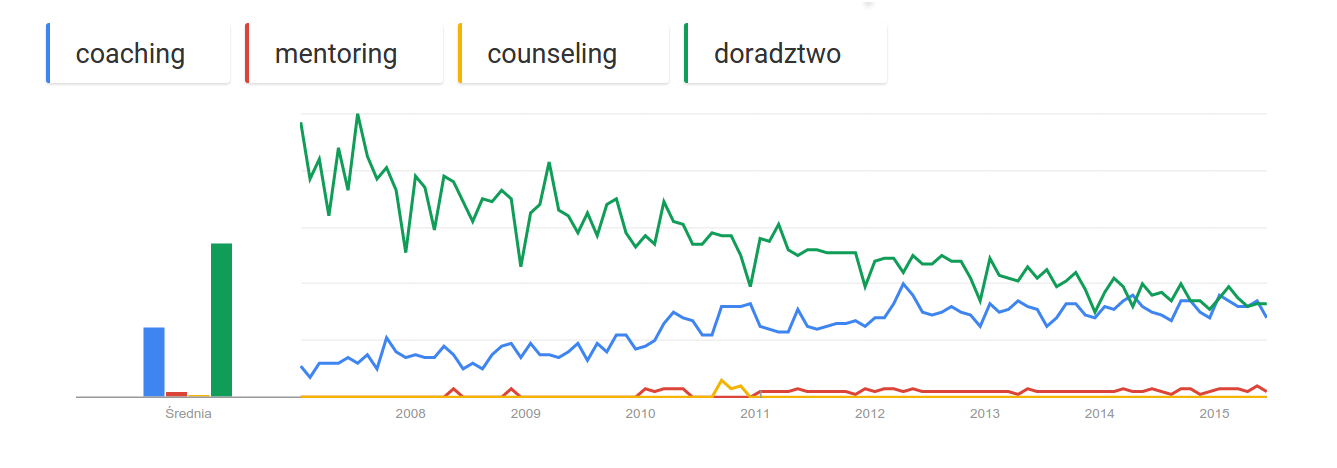
\includegraphics[width=17cm]{img/popularnosc}
  \caption{\TODO{opis}}
  \label{wykres}
\end{figure}

  \item Drugim szczególnie istotnym punktem w moim przeświadczeniu jest dyskrecja w sprawach dotyczących klienta.
      Cytując za Kodeksem Etycznym Izby Coachingu: "6.2 Jeśli dobro Klienta wchodzi w konflikt z lojalnością zawodową, Coach pracuje przede wszystkim dla dobra Klienta i postępuje zgodnie z uzgodnionym kontraktem.". Widocznym wnioskiem z tego punktu jest jak niezwykle ważne staje się czytelne ustalanie kontraktu pomiędzy coachem a klientem. Szczególna uwaga powinna mieć miejsce jeśli w proces zaangażowany jest również zewnętrzny zleceniodawca.
\end{itemize}

\subsection{Grupa docelowa procesu coachignowego}

\begin{itemize}
  \item im bardziej samodzielnym tym lepiej, ale przynajmniej w obszarze celów procesu
  \item osobom o wysokiej motywacji
  \item znajdującym się w nowej dla nich sytuacji (którym prawdopodobnie towarzyszy wysoka motywacja pozytywna) lub
       ulegających wypaleniu lub frustracji (wysoka motywacja negatywna). W drugim przypadku należy również rozważyć
       mentoring/szkolenia (np. frustracja wynika z braków wiedzy i przez to nie są osiągane efekty) lub consuelling \TODO{pisownia?}.
  \item dla osób stojących przed dylematem i aktywnie szukających jego rozwiązania
\end{itemize}

Tak jak zostało to podkreślone w poprzedniej sekcji - bardzo istotnym aspektem pracy coacha jest wiedza o tym, kiedy klient powinien
zostac skierowany do innego specjalisty. Przy pomocy tabeli \ref{table:kategorie} można zidentyfikować następujące przypadki:
\begin{itemize}
\item[--] W przypadku osoby potrzebującej wiedzy i gotowych rozwiązań - mentoring lub szkolenia.
\item[--] W przypadku osoby o niskiej motywacji / wypaleniu - consuelling.
\item[--] W przypadku osób stojących przed decyzją, ale nie dylematem - tzn. potrzebujących wiedzy i oceny sytuacji - pomoc konsultant.
\item[--] W przypadku osób w stanach depresyjnych, nie widzących możliwych rozwiązań i niskiej motywacji do wprowadzania zmian w swoim życiu - terapia.
\end{itemize}
